\documentclass[10pt]{standalone}
\usepackage{amsmath}
\usepackage{amssymb}
\usepackage[utf8]{inputenc}
\usepackage{pgf,tikz,pgfplots}
\pgfplotsset{compat=1.15}
\usetikzlibrary{arrows}
\pagestyle{empty}

\begin{document}

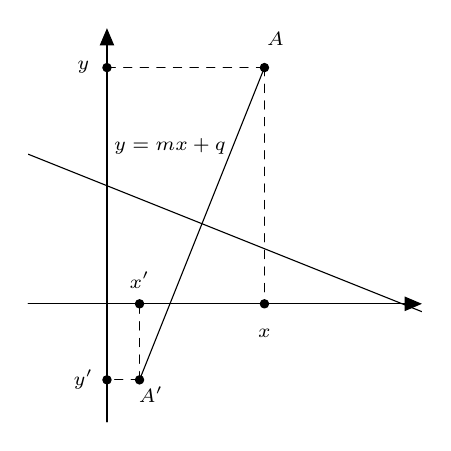
\begin{tikzpicture}[line cap=round,line join=round,>=triangle 45,x=1.0cm,y=1.0cm]
\draw[->] (-1.0,0.) -- (4.,0.);
;
\draw[->] (0.,-1.5) -- (0.,3.5);
\clip(-1.,-1.5) rectangle (4.,3.5);
\draw [domain=-1.:4.] plot(\x,{(--1.5-0.4*\x)/1.});
\draw [dash pattern=on 3pt off 3pt] (2.,3.)-- (2.,0.);
\draw  (2.,3.)-- (0.4137931034482758,-0.9655172413793105);
\draw [dash pattern=on 3pt off 3pt] (0.4137931034482758,-0.9655172413793105)-- (0.4137931034482758,0.);
\draw [dash pattern=on 3pt off 3pt] (0.,3.)-- (2.,3.);
\draw [dash pattern=on 3pt off 3pt] (0.4137931034482758,-0.9655172413793105)-- (0.,-0.9655172413793105);
\begin{scriptsize}
\draw[color=black] (-4.14,2.99) node {$f$};
\draw [fill=black] (2.,3.) circle (1.5pt);
\draw[color=black] (2.14,3.37) node {$A$};
\draw [fill=black] (0.4137931034482758,-0.9655172413793105) circle (1.5pt);
\draw[color=black] (0.56,-1.15) node {$A'$};
\draw [fill=black] (2.,0.) circle (1.5pt);
\draw[color=black] (2.0,-0.37) node {$x$};

\draw[color=black] (0.8,2.0) node {$y=mx+q$};
\draw [fill=black] (0.4137931034482758,0.) circle (1.5pt);
\draw[color=black] (0.4137931034482758,0.3) node {$x'$};

\draw [fill=black] (0.,3.) circle (1.5pt);
\draw[color=black] (-0.3,3.0) node {$y$};

\draw [fill=black] (0.,-0.9655172413793105) circle (1.5pt);
\draw[color=black] (-0.3,-0.9655172413793105) node {$y'$};

\end{scriptsize}

\end{tikzpicture}
\end{document}